%Experimental Results and Analysis – in this section, you should show the quantitative results – charts and tables. Analyze the results by explaining and highlighting what is important on them in terms of your goals and what is bad. You should explain the strange results too.

%V ďalšej časti prezentujte vlastný prínos a vlastné výsledky porovnajte s výsledkami iných. Charakterizujte použité metódy.
%Vyhýbajte sa používaniu žargónu.
%Používajte starú múdrosť: 1 obrázok je viac než 1000 slov.

%============================================================
\subsection{Complex binary vector associations} 
\label{sec:results-k3}

In this section, we analyse TLR~(\ref{sec:our-tlr}) and GeneRec~(\ref{sec:models-generec}) performance on the \emph{CBVA} task~(\ref{sec:datasets-k3}). The methodology is similar as in case of the 4-2-4 encoder task described in \ref{sec:results-auto4-introduction}. The main difference is that we tried several architectures of type 16-$n$-16 for $n \in \{3,\,4,\cdots,\,10\}$. Second difference is the setting of $Epoch_{\rm max}$ to 20,000 for TLR and 5,000 for GeneRec because the bigger network size. 

%============================================================
\subsubsection{Two learning rates} 
\label{sec:tlr-k3}

Comparison of success rate for different hidden sizes and $(\lambda_v,\,\lambda_h)$ pairs is shown in figure~(\ref{fig:results-tlr-k3-performance}). We see that TLR was able to learn the CBVA task only with 3 hidden neurons. The successfull values of ($\lambda_v, \lambda_h$) lie on the half line $[(1, 0.1), (10^4, 0.1)]$. This behaviour of TLR is similar to the behaviour of TLR on the \emph{4-2-4 encoder} task~(\ref{fig:results-bal-recirc-auto4-performance}). Again, the performance mostly depends on $\lambda_h$ and it is bounded by a value of $\lambda_v$. We observe that the perfect success space smoothly expands from top to down as increasing the hidden size. This is not true for GeneRec as shown in figure~\ref{fig:results-generec-k3-success}. 

%Main purpose of this dataset is to test different hidden sizes 
%======== (4D) L1 x L2 x patSuccF x hidden size =========
%======== (4D) L1 x L2 x epochs x hidden size =========

\begin{figure}[H]
  \centering
  %Hidden size = 3 \\
  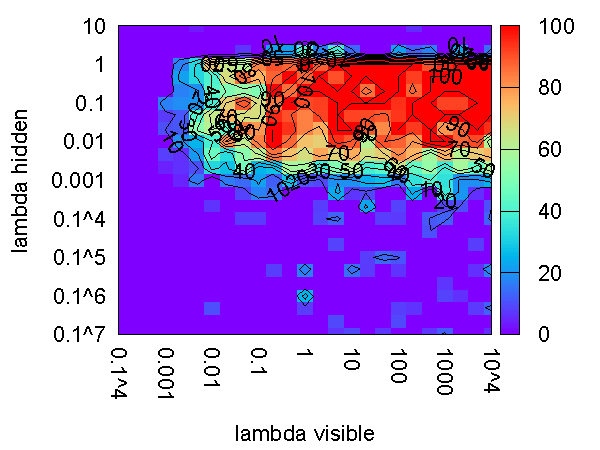
\includegraphics[width=0.49\textwidth]{img/k3/tlr-3-success.pdf} 
  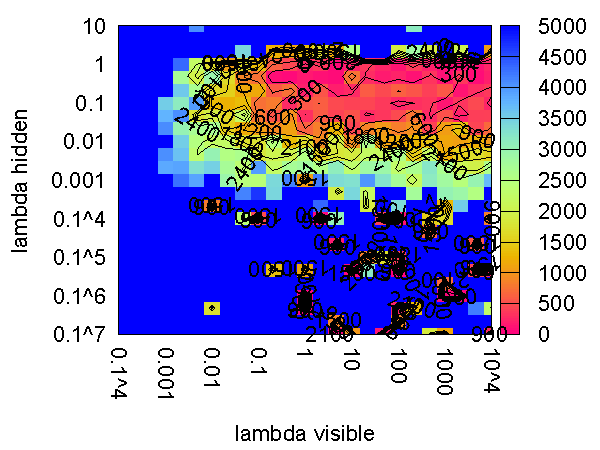
\includegraphics[width=0.49\textwidth]{img/k3/tlr-3-epoch.pdf}   
  %Hidden size = 4 \\
  %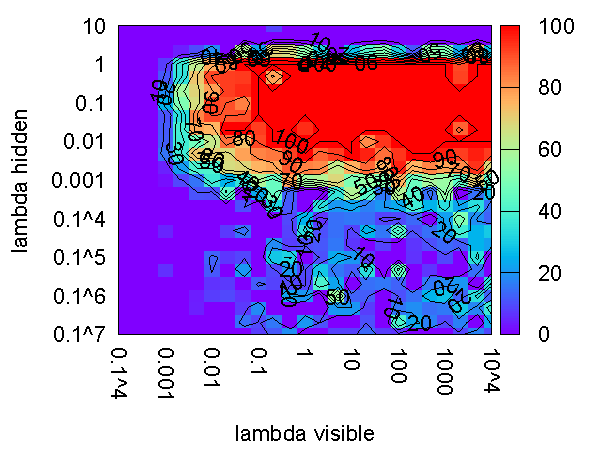
\includegraphics[width=0.49\textwidth]{img/k3/tlr-4-success.pdf} 
  %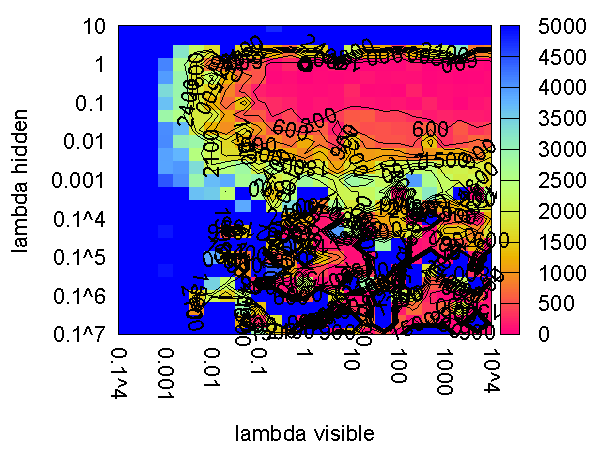
\includegraphics[width=0.49\textwidth]{img/k3/tlr-4-epoch.pdf}   
  %Hidden size = 5 \\
  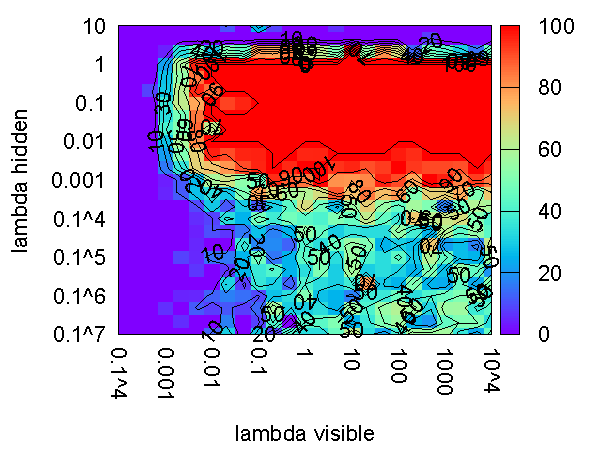
\includegraphics[width=0.49\textwidth]{img/k3/tlr-5-success.pdf}   
  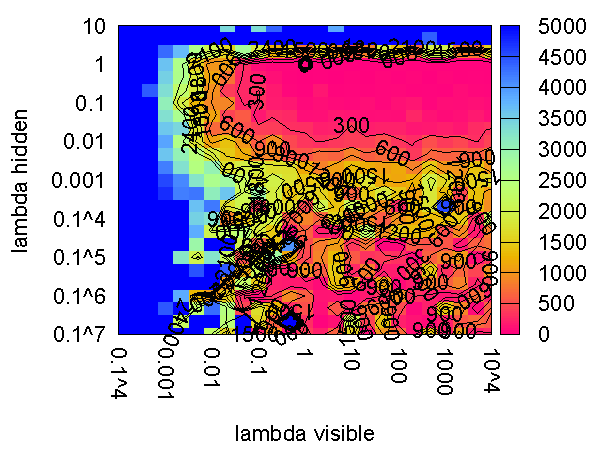
\includegraphics[width=0.49\textwidth]{img/k3/tlr-5-epoch.pdf}  
  %Hidden size = 8 \\
  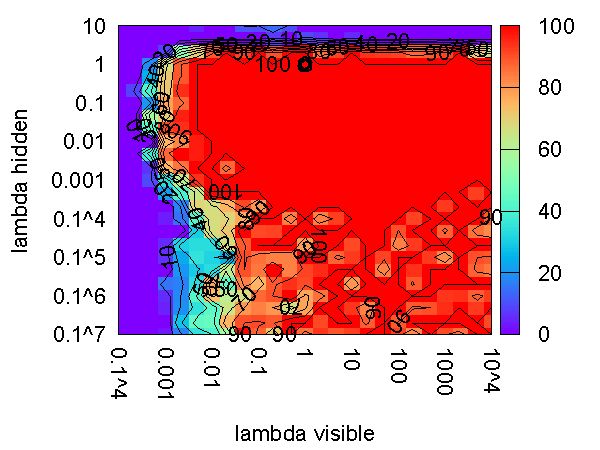
\includegraphics[width=0.49\textwidth]{img/k3/tlr-8-success.pdf} 
  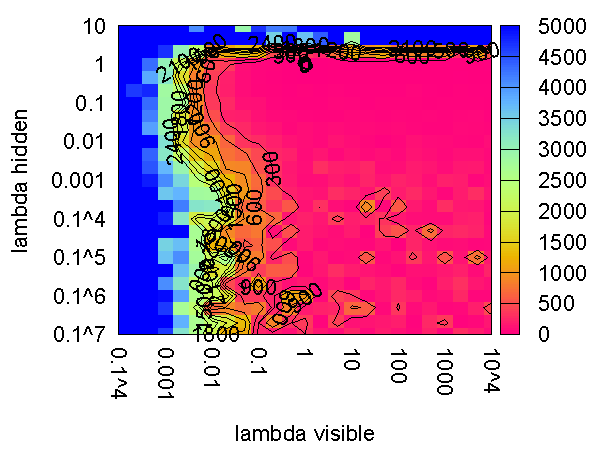
\includegraphics[width=0.49\textwidth]{img/k3/tlr-8-epoch.pdf}    
  \caption{TLR performance on the \emph{CBVA} task with hidden sizes 3, 5 and 8 from top to bottom.}
  \label{fig:results-tlr-k3-performance}
\end{figure}

Next we analysed the performance of TLR for best $\lambda_h$ and $\lambda_v$ in figure~\ref{fig:results-tlr-auto4-epoch}. We can observe that TLR is increasing its success rate in time steadily. Moreover, we see that the candidate selection~(\ref{sec:sim-exp-candidates}) has positive impact on the network performance.
Note that the CBVA task is non bijective, i.e.~one output has several inputs, therefore it is impossible to achieve 100\% $patSucc^B$ or $bitSucc^B$. 

%======== (3D) best TLR on ALL_SUCC x epoch (std-dev) x hidden size ==========
\begin{figure}[H]
  \centering
  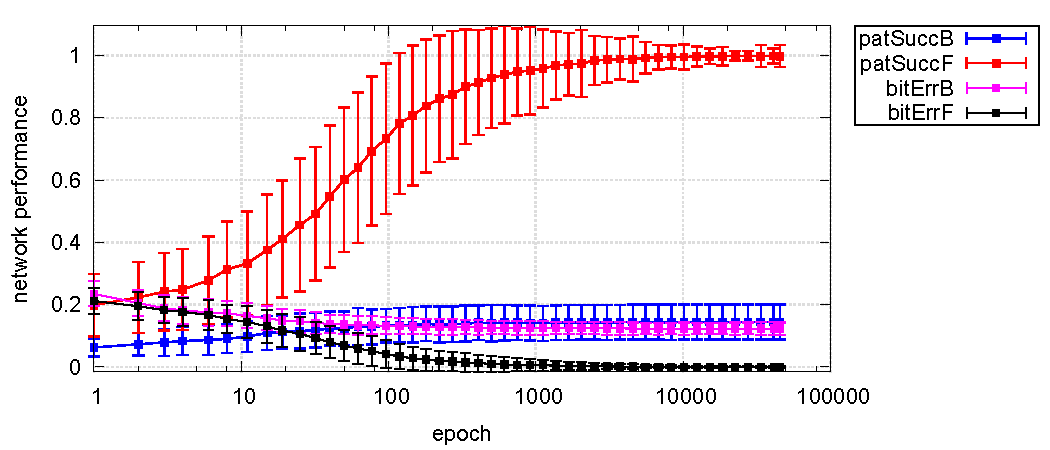
\includegraphics[width=0.8\textwidth]{img/tlr-k3-3-best-perf.pdf}   
  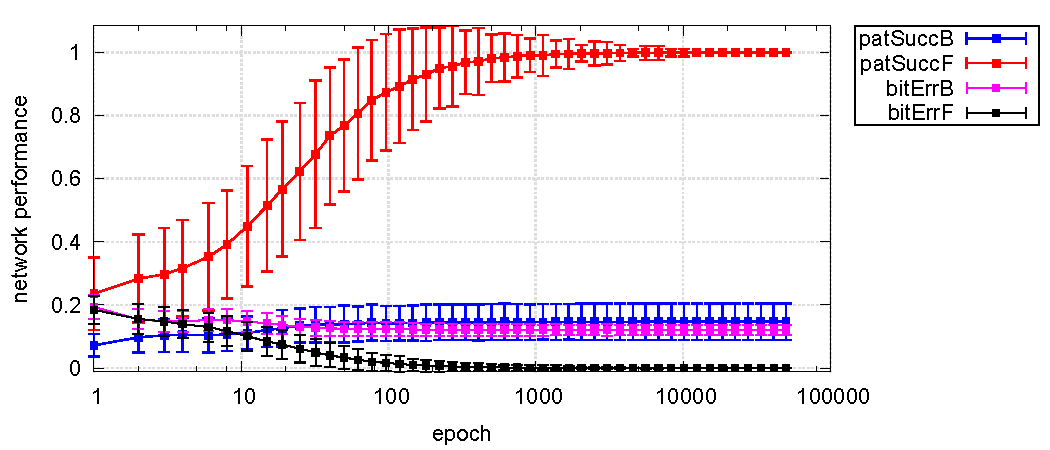
\includegraphics[width=0.8\textwidth]{img/tlr-k3-3-best-can.pdf}      
  \caption{TLR success rate timeline for the \emph{CBVA} task with $\lambda_h=0.1$ and $\lambda_v=100$. Top without candidate selection and bottom with candidate selection. }
  \label{fig:results-tlr-k3-epoch} 
\end{figure}

\subsubsection{Comparison} 
\label{sec:results-cmp-k3} 
Although CBVA is a higher dimensional problem than the 4-2-4 encoder problem, the networks were able to achieve perfect success rate and comparable convergence time as shown in table~(\ref{tab:results-cmp-k3}). The interesting fact is that having two learning rates has no advantage over setting $\lambda_h = \lambda_v$. This disproves our intuition that a more general model should achieve better. 

%===== table: best parameter setting networks with hidden.size= constant (success, epoch, stddev) / model \\

\begin{table}[H] 
  \centering
    \begin{tabular}{|l|l|l|l|l|}
    \hline
    Algorithm (section)&$\lambda_h$&$\lambda_v$&$patSucc^F$ &Epochs\\ %&SEM(success) \\
    \hline
    GR~(\ref{sec:models-generec}) & 0.1 & 0.1 & 100 & 84\\ %&28\\
    \hline
    GR TLR &0.03 & 1.0 & 100 & 89\\ %&28\\
    \hline
    BAL~(\ref{sec:models-bal})&0.5& 0.5&100& 54\\ %&2.0e+08\\
    \hline
    BAL TLR~(\ref{sec:our-tlr})&1.0& 5.0 & 100& 64\\ %&1.52e+08\\
    %\hline
    %BAL TLR Can~(\ref{sec:sim-exp-candidates})& & & & \\ %&5,070,000\\ 
    \hline 
    \end{tabular}
  \caption{Comparison of TLR and GeneRec on \emph{CBVA} using 3 hidden neurons.} 
  \label{tab:results-cmp-k3}
\end{table}

%SELECT lambda, lambda_ih, 100*AVG(success) AS 'suc', AVG(epoch) AS 'epc' FROM data WHERE epoch <> 0 GROUP BY lambda,lambda_ih ORDER BY suc ASC, epc DESC; 
%generec tlr H, V
%96.0 0.03 0.3
%96.0 0.1 0.3
%96.0 0.1 1.0
%98.0 0.003 0.1
%98.0 0.03 1.0

%generec pure 

%tlr pure 
%2.0|0.5|100.0|98.7777777777778
%2000.0|1.0|100.0|86.48
%5000.0|0.5|100.0|77.1428571428571
%5.0|1.0|100.0|64.0
%0.5|0.5|100.0|54.0

%tlr candidate 


\subsubsection{GeneRec} 

We used the two learning rate approach also for GeneRec. In figure~\ref{fig:results-tlr-k3-performance} we compare success rate for different values of $(\lambda_v,\, \lambda_h)$ and different hidden sizes. We can observe a similar behaviour for GeneRec with the 16-3-16 architecture as for the 4-2-4 encoder task~(\ref{fig:results-generec-auto4-performance}). That is the success space is bounded and the importance of both learning rates is same. Furthermore, as the hidden size becomes bigger, the success rate expands downwards as with TLR in figure~\ref{fig:results-tlr-k3-performance}. 

\begin{figure}[H]
  \centering
  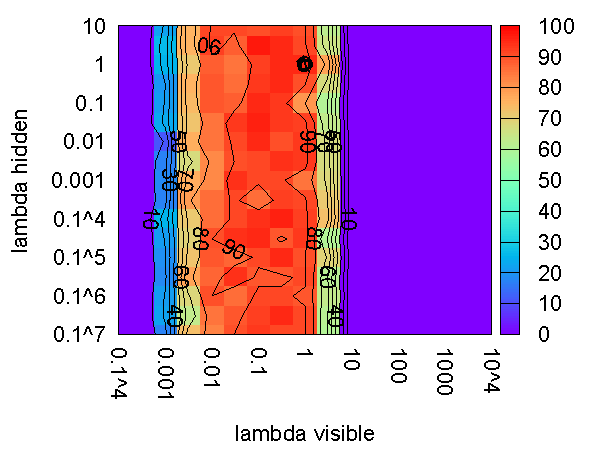
\includegraphics[width=0.45\textwidth]{img/k3/generec-3-success.pdf} 
  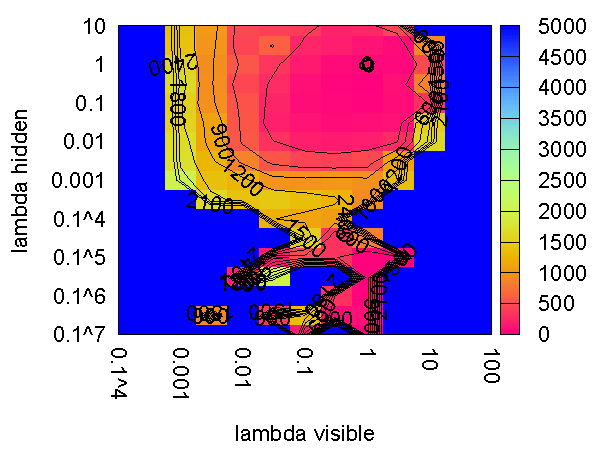
\includegraphics[width=0.45\textwidth]{img/k3/generec-3-epoch.pdf}   
%  Hidden size = 4 \\
%  \includegraphics[width=0.49\textwidth]{img/k3/generec-4-success.pdf} 
%  \includegraphics[width=0.49\textwidth]{img/k3/generec-4-epoch.pdf}  
  \includegraphics[width=0.45\textwidth]{img/k3/generec-6-success.pdf} 
  \includegraphics[width=0.45\textwidth]{img/k3/generec-6-epoch.pdf}  
%  Hidden size = 7 \\
%  \includegraphics[width=0.49\textwidth]{img/k3/generec-7-success.pdf} 
%  \includegraphics[width=0.49\textwidth]{img/k3/generec-7-epoch.pdf}    
  \caption{\emph{GeneRec} performance on the \emph{CBVA} task with hidden sizes 3 (top) and 5 (bottom).} %For greater hidden sizes the results were very similar to the results with hidden size 5.}
  \label{fig:results-generec-k3-success}
\end{figure}

